\documentclass[12pt]{book}
\usepackage{booktabs}
\usepackage[table]{xcolor}
\usepackage{tcolorbox}
\usepackage[T1]{fontenc}
\usepackage{wrapfig}
\usepackage{url}
\usepackage{dsfont}
\usepackage{enumitem}
\usepackage{array}
\usepackage{booktabs}

\usepackage{mathtools, nccmath}
\usepackage[polish]{babel}
\usepackage[utf8]{inputenc}
\usepackage{lmodern}
\usepackage{pifont}
\usepackage{blkarray, bigstrut}
\usepackage{amsmath}
\usepackage{kbordermatrix}
\usepackage{cases}
\usepackage{graphicx}
\usepackage{cellspace}
\usepackage[T1]{fontenc}
\usepackage{amsthm}
\selectlanguage{polish}
\usepackage{amsmath}
\usepackage{graphicx}
\usepackage{float}
\usepackage{cite}
\usepackage[margin=2.5cm]{geometry}
\theoremstyle{plain}
\newtheorem{definicja}{Definicja}
\newtheorem{twr}{Twierdzenie}
\newtheorem{lem}[twr]{Lemat}
\newtheorem{mur}{Murphy}[section]
\newcolumntype{P}[1]{>{\centering\arraybackslash}p{#1}}
\newcommand\green{\cellcolor{green!10}}
\newcommand\cincludegraphics[2][]{\raisebox{-0.5\height}{\includegraphics[#1]{#2}}}
\newcommand\red{\cellcolor{red!20}}
\newcommand\blue{\cellcolor{blue!20}}
\newcommand{\R}{\mathbb{R}}
\newcommand*{\tabbox}[2][t]{%
	\vspace{0pt}\parbox[#1][3.7\baselineskip]{1cm}{\strut#2\strut}}
\newcommand\addtag{\refstepcounter{equation}
	\renewcommand{\labelenumii}{\theenumii}
	\renewcommand{\theenumii}{\theenumi.\arabic{enumii}.}
	\tag{\theequation}}

\begin{document}
	\title{Optymalizacja  systemu sygnalizacji świetlnej w 
		oparciu o przepływowy model ruchu pojazdów.}
	\author{Michał Lis}
	\date{\today}
	\maketitle
	\tableofcontents
	
	\chapter {środowiska symulacyjne qwe}
	\section{Srodowisko 4}
	\begin{figure}[H]
		\centering
		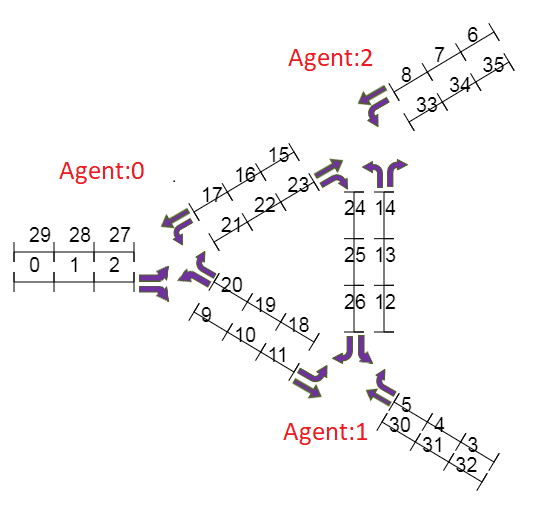
\includegraphics[width=10cm]{env_4_agenci}
		\label{fig:env_4_agenci}
		\caption{środowisko 4}
	\end{figure}
	
	środowisko posiada 12 jednokierunkowych dróg. Każda droga ma 3 odcinki co daje w sumie 36 odcinków (są numerowane od 0 co widać na rysunku \ref{fig:env_4_agenci}).
	W sieci dróg znajdują się 3 skrzyżowania. Do każdego z nich jest przypisany agent, który odpowiada za sterowanie sygnalizacją świetlną.
	Pojazdy w jednym interwale czasowym pokonują jeden odcinek. Na skrzyżowaniach w przypadku zielonego światła przejeżdża maksymalnie 10 pojazdów w jedną stronę.
	
	
	\begin{figure}[H]
		\centering
		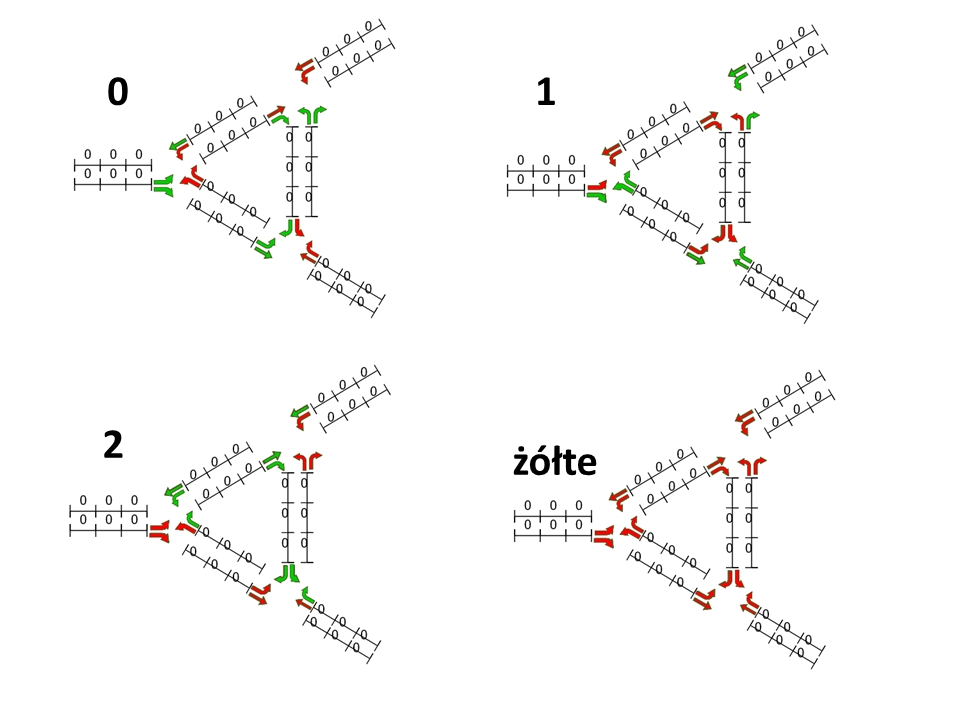
\includegraphics[width=14cm]{env_4_fazy}
		\label{fig:env_4_fazy}
		\caption{środowisko 4 - fazy świateł}
	\end{figure}
Fazy świetlne: Każde skrzyżowanie posiada 4 fazy świetlne przedstawione powyżej. Fazy 0, 1 i 2 posiadają pewne zielone światła. Agent podejmuje decyzję o zmianie tych trzech faz. Zmiana faz świateł nie jest natychmiastowa i następuje dopiero po 2 interwałach czasowych fazy żółtych świateł. Agent może podjąć akcję a należącą do
[0,1,2] w przypadku gdy obecna faza f należy do [0,1,2]. W pozostałym przypadku agent jest zobowiązany do przekazania akcji 'yellow'.

\section{Uczenie srodowiska 4}	
\subsection{Podejście 1}
Każdy z trzech agentów jako stan przyjmuje 10 elementowy wektor. 9 elementów to ilości pojazdów na odcinkach będących przed skrzyżowaniem przypisanym do agenta. Wektor uzupełnia wartość obecnej fazy. 
Nagrody dla danego stanu sa przyznawane jako suma pojazdów, które przejechały przez skrzyżowanie w trakcie najbliższych 4 interwałów czasowych. Początkowo przeprowadzana jest symulacja 100 epizodów z czego każdy trwa 90 interwałów czasowych. Ma ona na celu wygenerowania danych do treningu. Do nauki agent zapamiętuje jedynie te stany, których faza to 0, 1 lub 2. Nieistotne w procesie uczenia są stany z fazą 'yellow' gdyż agent ma tylko 1 możliwą decyzję do podjęcia. Następnie trenowana jest sieć neuronowa przyjmująca na wejście stan - 10 elementowy wektor. Sieć na wyjściu zwraca 3-elementowy wektor określający przewidziane nagrody dla akcji podjętej w zadanym stanie.
Podsumowując dla wybranego agenta:
\begin{itemize}
\item \textbf{Stanem} są ilości pojazdów przed skrzyżowaniem oraz aktualna faza świetlna
\item \textbf{Nagrodą} w chwili t jest suma pojazdów, które przejechały przez skrzyżowanie w trakcie najbliższych 4 interwałów czasowych czyli do momentu t+4.
\item \textbf{Dane} są generowane poprzez przeprowadzenie 100 symulacji (każda ma 90 interwałów czasowych).
\item \textbf{Sieć neuronowa} na podstawie wygenerowanych danych przewiduje najlepszą akcję dla obecnego stanu
\item Końcowa symulacja zostaje przeprowadzona wedle przewidzianych przez sieć neuronową najlepszych akcji
\end{itemize}

\end{document} 

















\chapter{Przedstawienie problemu optymalizacyjnego}

\bibliographystyle{IEEEtran}

\chapter{Przegląd metod optymalizacyjnych}
\section{Kategorie uczenia maszynowego}
Uczenie maszynowe to dziedzina wchodząca w skład nauk zajmujących się sztuczną inteligencją. Samo uczenie w najprostszym kształcie może być rozumiane jako dobór parametrów na podstawie dostępnych danych. Uczenie maszynowe jest powszechnie dzielone na 3 kategorie nauki \cite{machineLearningClassification}.
\begin{enumerate}
	\item \textbf{Nadzorowane} \\
	Dane używane do uczenia nazywane są zbiorem treningowym. Każdy pojedynczy element zbioru treningowego ma informacje wejściowe oraz pewną pożądaną wartość wyjściową. W trakcie uczenia algorytm dopasowuje swoje parametry tak aby na podstawie danych wejściowych mógł przewidzieć wartość wyjściową. Przykładami uczenia nadzorowanego jest np. rozpoznawanie tekstu pisanego, detekcja obiektów na zdjęciach.
	\item \textbf{Nienadzorowane}
	Uczenie nienadzorowane różni się od nadzorowanego tym, że nie  są znane pożądane wartości wyjściowe. Celem nauki jest na podstawie podobieństw poszczególnych elementów zgrupowanie ich do odpowiednich klas. Przykładem uczenia nienadzorowanego może być np. klasyfikacja gatunków drzew na podstawie wiedzy o ich wysokościach i szerokości korony drzew.
	\item \textbf{Wzmocnione}
	W środowisku uczenia ze wzmocnieniem istnieje agent, który jest odpowiedzialny za podejmowanie pewnych decyzji. Każda decyzja ma wpływ na stan środowiska, które zwraca agentowi nagrodę. Celem uczenia ze wzmocnieniem jest ustalenie strategii maksymalizującej skumulowaną wartość nagród.
\end{enumerate}
Ze wszystkich trzech kategorii uczenie ze wzmocnieniem odpowiada problemowi rozważanym w rozdziale Y. Szczegółowy opis uczenia ze wzmocnieniem zostanie przedstawiony w następnej sekcji.
\section{Uczenie ze wzmocnieniem}
Schemat uczenia ze wzmocnieniem składa się z następujących elementów:
\begin{enumerate}
	\item \textbf{Agent} jest odpowiedzialny za podejmowanie pewnych decyzji. Ma on wiedzę na temat obecnego stanu środowiska i otrzymuje w każdym kroku czasowym sygnał nagrody. Jego decyzje wpływają na stan środowiska.
	\item \textbf{Środowisko} jest przestrzenią posiadającą dynamiczny stan widoczny dla agenta. Chociaż to agent podejmuje akcje, to środowisko ma zdefiniowany model zmiany stanu. Model zmiany stanu może być stochastyczny oraz niewidoczny dla agenta. Oznacza to, że dwie te same akcje podjęte w tym samym stanie nie zawsze przyniosą identyczny następny stan. Innymi słowy agent nie może być stuprocentowo pewny rezultatów swoich akcji. Środowisko jest także nadawcą sygnału nagrody.
	\item \textbf{Strategia} definiuje sposób doboru akcji przez agenta w danej chwili. Jest to funkcja, która przyjmuje stan środowiska i zwraca akcje, która ma być przeprowadzona. 
	\item \textbf{Sygnał nagrody} definiuje cel problemu uczenia ze wzmocnieniem. W każdym kroku czasowym środowisko wysyła agentowi liczbę rzeczywistą, która jest nazywana nagrodą(reward). Wartości nagród są czynnikiem wpływającym na zmianę strategii, gdyż zadaniem agenta jest maksymalizacja nagród. Wartość nagród zatem definiuje, które zdarzenia są dobre, a które złe dla agenta. Biologicznym odpowiednikiem dodatniej nagrody jest przyjemność, a ujemnej - ból. 
	\item \textbf{Funkcja wartości} zwraca wartość stanu czyli oczekiwaną sumę nagród jakie agent osiągnie w przyszłości będąc aktualnie w tym stanie. 
\end{enumerate}
\begin{figure}[H]
	\centering
	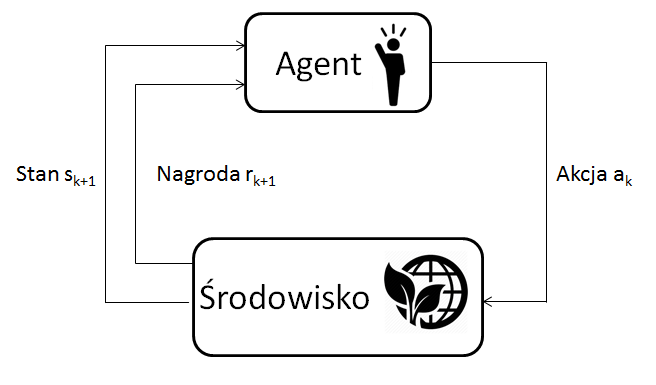
\includegraphics[width=14cm]{agent-srodowisko}
	\caption{Interakcje pomiędzy agentem a środowiskiem.}
	\label{fig:agent-srodowisko}
\end{figure}
\newpage
Algorytmy uczenia ze wzmocnieniem zazwyczaj stosuje się do rozwiązywania problemu procesu decyzyjnego Markowa. Sam \textbf{proces decyzyjny Markowa} jest zdefiniowany jako uporządkowana czwórka $(S,A,P_a,R_a)$, gdzie:
\begin{enumerate}
	\item $S$ to zbiór stanów
	\item $A$ to zbiór akcji. Notacją $A_s$ oznaczane są możliwe akcje dla stanu $s$.
	\item $P_a(s,s')=Pr(s_{t+1}=s'|s_t=s,a_t=a)$ to prawdopodobieństwo, że akcja $a$ wykonana w stanie $s$ w chwili $t$ doprowadzi do stanu $s'$ w chwili $t+1$.
	\item $R_a(s,s')$ to oczekiwana nagroda otrzymana w wyniku akcji podjętej w stanie $s$ prowadzącej do stanu $s'$.
\end{enumerate}

Problemem procesu decyzyjnego Markowa jest odnalezienie optymalnej strategii. Strategia określona jest jako funkcja $\pi(s)$ przyjmująca jako argument stan, a zwracająca podejmowaną akcję. Celem optymalizacji jest odnalezienie strategii maksymalizującej wartość:
\[
G=\sum_{k=0}^{K} \gamma^k R_{k} \addtag \label{eq:Markov_maximize}
\]
Chociaż strategii $\pi(s)$ nie ma we wzorcze \ref{eq:Markov_maximize}, to strategia wpływa na otrzymywane nagrody $R_{k}$ w każdej chwili $k$.\\
$\gamma \in (0,1]$ jest czynnikiem dyskontującym. Idea dyskontowania nagród zaczerpnięta jest z rachunku finansowego. Przykładowo wpływ 1000 złotych po upływie roku czasu jest z pewnością bardziej wartościowy niż za 20 lat. Innymi słowy - pieniądze są liczone w czasie i tak samo należy postępować z nagrodami. Im wartość $\gamma$ jest bliższa 0 tym bardziej istotne są początkowe nagrody. Dla $\gamma=1$ wszystkie nagrody są równie istotne - bez względu na czas ich otrzymania.\\
Analogicznie do (\ref{eq:Markov_maximize}) jest ustalona funkcja wartości stanu. Jako wartość stanu $s$ określone jest:
\[
G_t=\sum_{k=t}^{K} \gamma^k R_{k}=R_{t}+\gamma R_{t+1}+\gamma^{2} R_{t+2}+...+\gamma^{K}R_K \addtag \label{eq:Markov_state_value_G}
\]
Zostanie przedstawiony teraz przykład obliczeniowy. Agent podejmuje decyzje na których podstawie otrzymuje ciąg  nagród $R_0=0, R_1=2,R_2=6,R_3=-1,R_4=2,R_5=1$. Czynnik dyskontujący $\gamma$ jest równy 0,9. Jaka jest wartość $G$ oraz $G_1,G_2,G_3,G_4,G_5$?\\
\begin{figure}[H]
	\centering
	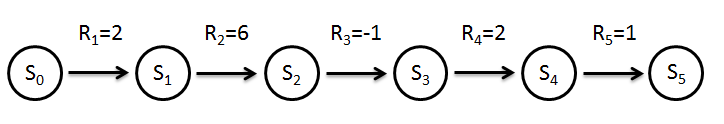
\includegraphics[width=14cm]{rewards-graph}
	\caption{Ciąg nagród i stanów.}
	\label{fig:agent-srodowisko}
\end{figure}\noindent
Najłatwiej obliczenia rozpocząć od $G_5$, ponieważ
\[G_{t}=R_{t}+\gamma G_{t+1} \label{eq:G_reccurential} \addtag \].\\
$G_5=R_5=1$.\\
$G_4=R_4+\gamma G_{5}=\;\;2+0,9\cdot 1=2,9$\\
$G_3=R_3+\gamma G_{4}=\!-1+0,9\cdot2.9=1,61$\\
$G_2=R_2+\gamma G_{3}=\;\;6+0,9\cdot1,61 \approx 7,45$\\
$G_1=R_1+\gamma G_{2}=\;\;2+0,9\cdot 7,45 \approx 8,70$\\
$G\;\,=R_0+\gamma G_{1}=\;\;0+0,9\cdot 8,70 \approx 7,83$\\

\section{Programowanie dynamiczne}
Termin programowania dynamicznego odnosi się do algorytmów wyliczających optymalne strategie procesu decyzyjnego Markowa w przypadku posiadanej całkowitej wiedzy na temat modelu środowiska\cite{reinforcementBook}. Środowisko nie musi być w pełni deterministyczne tzn. nie za każdym razem akcja przeprowadzana ze stanu $s_k$ musi w efekcie doprowadzić do tego samego stanu $s_{k+1}$. Jednak w takim przypadku musi być znany rozkład prawdopodobieństwa przydzielania nowego stanu na podstawie poprzedniego i właśnie podjętej przez agenta akcji. Dodatkowo wymagana jest możliwość ustalenia dowolnego stanu w trakcie uczenia. \\ Początkowa strategia $\pi(s)$ jest dowolna, najczęściej losowa.
Przedstawiony algorytm jest podzielony na 2 części. Część predykcji(prediction) oraz kontroli (control). 
\\\textbf{Proces predykcji} ma za zadanie ustalenie wartości stanów na podstawie ustalonej strategii. Jej algorytm jest następujący:
\begin{enumerate}
	\item{Przyjmij daną z góry $\pi$ jako strategię podejmowania akcji}
	\item{Zainicjuj tablicę wartości stanów $V(s)$. Dla wszystkich możliwych stanów $s \in S$ przyjmij wartość $0$.}
	\item{$\Delta=0$}
	\item{Dla każdego $s \in S$:}
	\begin{enumerate}
		\item $v=V(s)$
		\item $V(s)=\sum_{s'}Pr(s'|s,\pi(s))[r+\gamma V(s')]$
		\item $\Delta = max(\Delta,|v-V(s)|)$
	\end{enumerate}
	\item Jeśli $\Delta< \theta$ to wróć do 3
	\item Zwróć $V(s)$ jako tablicę wartości stanów $V_{\pi}(s)$ dla strategii $\pi$.
\end{enumerate}
Parametr $\theta \geq 0$ definiuje w kroku 5. moment stopu. \\
Wartość $Pr(s',s,\pi(s))$ to prawdopodobieństwo, że akcja $\pi(s)$ podjęta w stanie $s$ doprowadzi do stanu $s'$. Z kolei $r$ jest właśnie otrzymaną nagrodą.
\\ Algorytm \textbf{kontroli} ma za zadanie odnaleźć bardziej optymalną strategię niż dotychczas. Jako argument przyjmuje on wyliczoną właśnie tablicę wartości stanów $V_{\pi}(s)$. Wprowadzona zostaje macierz $Q_{\pi}(s,a)$. Jest ona zdefiniowana następująco:
\begin{equation}
\begin{split}
Q_{\pi}(s,a) &= E[R_{t+1}+\gamma v_{\pi}(S_{t+1}) | S_t=s, A_t=a]  \\
&= \sum_{s'}Pr(s'|s,a)[r+\gamma V_{pi}(s')] 
\end{split}
\end{equation}
Oczywistym minusem tego algorytmu jest konieczność przeiterowania wszystkich stanów. W przypadku gdy stanów jest bardzo dużo algorytm staje się nieopłacalny.
Macierz przedstawia wartość akcji $a$ podjętej w stanie $s$. Algorytm kontroli jest następujący:
\begin{enumerate}
	\item{Przyjmij wyliczoną przez algorytm predykcji macierz wartości stanów $V_{\pi}(s)$}
	\item{Zainicjuj tablicę wartości stanów $V(s)$. Dla wszystkich możliwych stanów $s \in S$ przyjmij wartość $0$.}
	\item{$policy\_stable=false$}
	\item{Dla każdego $s \in S$:}
	\begin{enumerate}
		\item $old\_action=\pi(s)$
		\item $\pi(s)=argmax_{a\in A_s} \sum_{s'}Pr(s'|s,a)[r+\gamma V(s')]$
		\item Jeśli $old\_action \neq \pi(s)$ to $policy\_stable = true$
	\end{enumerate}
	\item Jeśli $policy\_stable=true$ to zwróć strategię $\pi(s)$.
\end{enumerate}
\section{Metoda Monte Carlo On-Policy}
Metody Monte Carlo są szeroką klasą algorytmów, których wyniki oparte są o losowe próbkowanie. Nie potrzebują one żadnej wiedzy na temat środowiska - akceptowalne są zarówno środowiska deterministyczne jak i stochastyczne. Algorytmy Monte Carlo uczenia ze wzmocnieniem są dzielone na dwie kategorie - On-Policy oraz Off-policy. W pracy zostanie przedstawiona metoda on-policy, która różni się od off-policy jedynie sposobem doboru momentu eksploracji. Metoda on-policy zakłada, iż ustalana jest pewna liczba $\epsilon$ bliska zeru. Określa ona prawdopodobieństwo kroku eksploracji, czyli wyboru losowej akcji. Pozostałe akcje są wybierane w sposób zachłanny, czyli podejmowana jest najbardziej wartościowa dostępna akcja. Algorytm przedstawiony jest poniższym pseudokodem.
\begin{enumerate}
	\item Zainicjuj słowniki:
	\begin{enumerate}
		\item $Q(s,a)$ - Wartość określa opłacalność wyboru akcji a w stanie s
		\item $Returns(s,a)$ - Wartość słownika to tablica wartości $G$ wyliczonych na podstawie otrzymanych reward'ów oraz wzoru (\ref{eq:Markov_state_value_G}).
		\item $\pi(s)$ - Określa jaka akcja ma zostać podjęta dla stanu s. Początkowo wszystkie akcje są wybrane losowo.
	\end{enumerate}
	\item Zasymuluj pełny epizod wedle strategii $\pi$
	\item Dla każdego stanu s i akcji a, które pojawiły się w epizodzie
	\begin{enumerate}
		\item Wylicz $G$ rekurencyjnie wedle wzoru (\ref{eq:G_reccurential})*
		\item Do tablicy Returns(s,a) dodaj wartość $G$
		\item $Q(s,a)=avg(Returns(s,a))$
		\item $\pi(s)=argmax_{a\in{A}}Q(s,a)$. Chyba, że wylosowany został krok ekspolarcji, wtedy $\pi(s)$ jest losowo wybraną akcją $a \in A$.
	\end{enumerate}
\end{enumerate}
*(Rozsądnym jest iterowanie w 3 kroku w kolejności odwrotnej do chronologicznej, gdyż ułatwia wykorzystanie wzoru (\ref{eq:G_reccurential}))
\\ Warto zauważyć następujące zalety metody Monte Carlo, których nie zapewniał algorytm programowania dynamicznego:
\begin{enumerate}
	\item Brak potrzeby wiedzy na tematu modelu
	\item Nie wymaga często nierealnego założenia, iż stan środowiska może zostać sztywno ustalony przez programistę. Wymagana jest jedynie możliwość przeprowadznia pełnych epizodów, co jest nieporównywalnie słabszym założeniem.
	\item Dobre skalowanie dla dużej przestrzeni stanu. Więcej czasu treningowego jest poświęcane dla stanów, które są często odwiedzane. Z kolei te, które nie pojawiają się prawie wcale - nie marnują dużo czasu w procesie nauki.
\end{enumerate}

\chapter{Optymalizacja sygnalizacji świetlnej}
\bibliography{refs}
\end{document}
